%!TEX root = ../report.tex

\section{Beweglichkeit}

Definition Beweglichkeit: Beweglichkeit ist die motorische Fähigkeit, Bewegungen willkürlich mit der erforderlichen Schwingungsweite ausführen zu können.

Verwandte Begriffe: \textbf{Gelenkigkeit} = Schwingungsweite von Gelenken, \textbf{Dehnfähigkeit} = Dehnbarkeit von Muskeln und Sehnen

Optimalitätseigenschaft: Stabilität versus Mobilität, Hypo- versus Hypermobilität

\subsection{Systematik und Determinanten}

\subsubsection*{Dimensionen }

\begin{minipage}{0.7\textwidth}
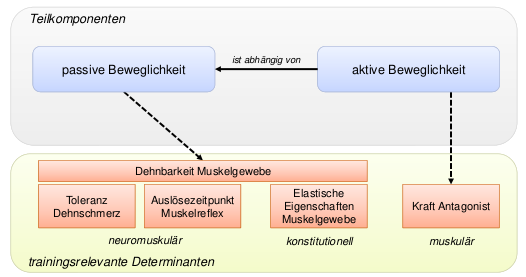
\includegraphics[width=\textwidth]{pictures/beweg_determinanten4}
\end{minipage}
\begin{minipage}{0.3\textwidth}
\begin{itemize}
    \item Passive Beweglichkeit: Beweglichkeit die unter Einwirken einer externen Kraft erreicht wird (z.B. Spagat, Schwerkraft)
    \item Aktive Beweglichkeit: Beweglichkeit, die durch aktive Muskelarbeit erreicht wird (z.B. Armschwung, Schuss, Spagatsprung)
\end{itemize}
\end{minipage}

Methoden im Beweglichkeitstraining:
\begin{itemize}
    \item aktiv: Antagonisten bewirken Dehnung
    \item passiv: Partner, Schwerkraft, andere Muskeln bewirken Dehnung
    \item statisch: langsames Einnehmen der Dehnposition, ohne Auslösung des Muskelreflexes (intensiv)
    \item dynamisch: schnelles, federndes Einnehmen der Dehnposition, mit (unter Inkaufnahme der) Auslösung des Muskelreflexes
\end{itemize}

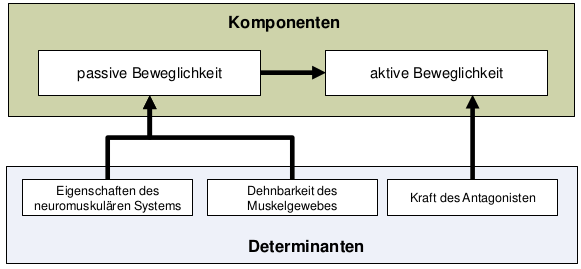
\includegraphics[width=0.9\textwidth]{pictures/beweg_determinanten2}

\subsubsection*{Muskelreflex}

Schnelle Bewegungen lösen den Muskelreflex aus, aber das Auslösen des Muskelreflexes ist kontraproduktiv zur Absicht der Dehnung. Wenn die Dehnung intensiv sein soll, sollte Muskelreflex nicht (nur minimal) ausgelöst werden, d.h. keine schnellen Bewegungen.

Der Muskeltonus ist Ausdruck des systemischen Erregungszustandes. Zu hoch impliziert sanfte Dehnung und Entspannungsübungen, zu niedrig dagegen intensive Dehnung.

Allgemein:
Ein Gelenk besteht aus Muskeln und Sehnen, Knochen, Knorpel und der Gelenkkapsel mit Bändern.
Es gibt verschiedene Rezeptoren:
\begin{itemize}
    \item Ruffini-Körperchen sind Mechanorezeptoren in Kapsel und Haut und reagieren auf Druck und Dehnung. Dabei registrieren sie das Ausmaß und die Geschwindigkeit von Gelenkbewegungen.
    \item Vater-Pacini-Körperchen sind Mechanorezeptoren im Gelenkbindegewebe und registrieren Beschleunigungen.
    \item Golgi-Sehnenorgan sitzt im Übergang zwischen Muskeln und Sehnen und registriert dort die Muskelspannung. Unter Umständen gibt es eine Reflexantwort.
    \item Muskelspindeln sind quergestreifte Muskelfasern, die ebenfalls als Mechanorezeptoren dienen. Sie lösen den Eigenreflex aus und messen das Ausmaß und die Geschwindigkeit einer Muskelbewegung.
\end{itemize}

\subsubsection*{Determinanten}

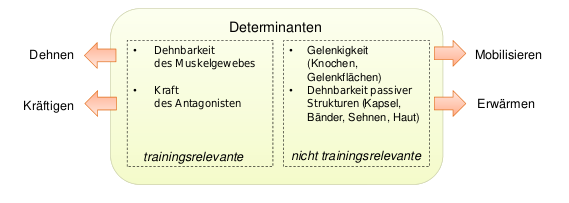
\includegraphics[width=\textwidth]{pictures/beweg_determinanten3}

\begin{minipage}{0.4\textwidth}
Entscheidend sind folgende anatomische Eigenschaften:
\begin{itemize}
    \item Freiheitsgrade und Funktionstüchtigkeit der Gelenke
    \item Bandhafte- und kapsuläre Hemmung
    \item Titinfilamente (hauptsächlich verantwortlich für Widerstand)
    \item Tendo-muskuläre Reflexschaltungen (Hemmungen)
\end{itemize}
\end{minipage}
\begin{minipage}{0.6\textwidth}
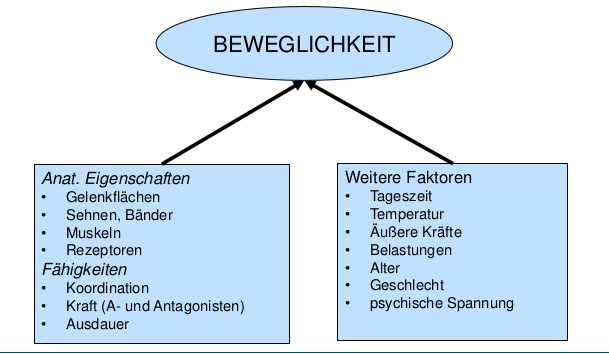
\includegraphics[width=\textwidth]{pictures/beweg_determinanten}
\end{minipage}
Weitere Einflussfaktoren:
\begin{itemize}
    \item Alter: Abnahme der Elastizität (H 2 O-Verlust; Weniger Zellen)
    \item Geschlecht: Einfluss des Östrogens
    \item Ausdauer: Kein Beweglichkeitstraining im Ermüdungszustand
\end{itemize}

\subsection{Bedeutung}

Beweglichkeit kann Bestandteil von Wettkampfleistungen sein (Bsp: bessere Bepunktung von Spagat in der Gymnastik) oder Voraussetzung für Wettkampfleistungen, konditionelle Fähigkeiten oder Teilleistungen sein (Bsp: bessere performance von beweglicheren Fußballspielern).

Als Beweglichkeitsreserve bezeichnet man die Differenz zwischen erforderlichem und maximalem Bewegungsausschlag. Eine große Reserve ist erstrebsam, weil dann nicht bis an die Dehnbarkeitsgrenze belastet werden muss (Ökonomisierung) und die Bewegung unter geringerem Widerstand ablaufen kann. Auch im Fitness- und Gesundheitstraining ist Dehnen zur Vermeidung von Dysbalancen und Verkürzungen relevant.

\subsubsection*{Aufwärmen vs Dehntraining}

Seit Mitte der 90er Jahren ist bekannt, dass intensives statisches Dehnen (Stretching) in der Aufwärmphase genau das Gegenteil von dem, was man sich erhofft, bewirkt.
Statt leistungssteigernd und verletzungsmindern zu wirken, führt es zu geringerer Leistung und einem größerem Verletzungsrisiko. Ausmaß: 4-8\% weniger vertikale Sprungleistung und 5-10\% Reaktivkraftleistungen

Gründe:
\begin{itemize}
    \item Geringere Kraftproduktion Muskel-Sehnen-Komplex (Verlängerung, Belastung der fibrillären Strukturen)
    \item Periphere neuromuskuläre Veränderungen, z.B. Reduktion der
    \item Erregbarkeit der Motoneurone
    \item Zentrale psychophysiologische Desaktivierungsprozesse, Senkung der zentralen Aktivierung
\end{itemize}

Verletzungsprophylaxe: Kräfte bei passiver Dehnung können sehr groß und unphysiologisch werden, zusätzliche steht ein epidemiologischer Nachweis der Verletzungsprophylaxe-Wirkung von intensivem Dehnen noch aus. Muskelkater kann durch (zu) intensives Dehnen verschlimmert bzw. sogar herbeigeführt werden...

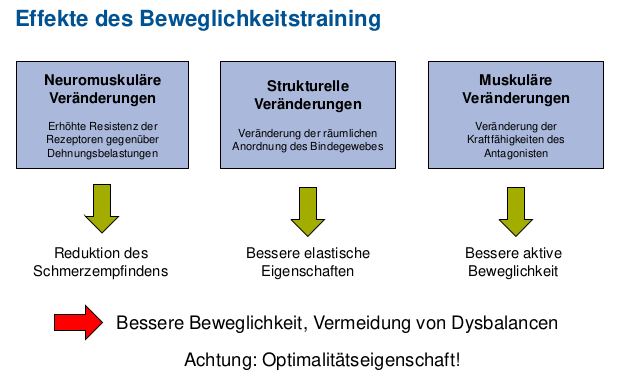
\includegraphics[width=0.9\textwidth]{pictures/beweg_effekte}

\subsection{Diagnostik}

Motorische Beweglichkeits-Tests z.b. mit ablesen auf einer Zentimeterskala und abgleich gegen Normtabelle. Problem von Normwerten: Liefern nur erste Hinweise

Ein anderes klassisches Verfahren zur einfachen Bestimmung von Beweglichkeitseinschränkungen in der Muskulatur  ist der Janda-Test.
Beispiel für den Hüftlendenmuskel: Rückenlage, Oberschenkel beugen und Richtung Brust heranziehen, dabei muss die Lendenwirbelsäule komplett aufliegen.
Anzeichen für Beweglichkeitseinschränkung: der Oberschenkel der Gegenseite geht nach oben.

\subsection{Trainingsmethoden}

\paragraph*{Belastungsnormative}
Problem: Wie wählt man die Intensität? \% des maximalen Bewegungsumfangs? Subjektives Rating über Schmerzskala?
Dauer, Umfang, Dichte, Häufigkeit weniger wichtig, entscheidend ist die Ausführungsart.

Ausführungsarten:
\includegraphics[width=0.9\textwidth]{pictures/beweg_ausführungsarten}

Static Stretching (SS):
\begin{itemize}
    \item Langsame Heranführung an Bewegungsgrenze bewirkt Hemmung des Dehnungsreflexes der Muskeln und Sehnenspindeln
    \item Einnehmen der Dehnposition, so dass deutliche
    Spannung spürbar ist ( = Andehnen).
    \item Wenn das Spannungsgefühl nachlässt, Verstärkung der Dehnung und erneutes Halten ( = Nachdehnen).
    \item Dauer: zwischen 5s und > 60s (je nach Trainingsziel)
\end{itemize}

Contract Relax (CR):
\begin{itemize}
    \item vorgeschaltete Kontraktion des Agonisten führt zur Hemmung des Dehnungsreflexes des Agonist (autogene Hemmung)
    \item Isometrische Kontraktion (submaximal bis maximal) des Agonisten (5s) (C=Contract)
    \item Entspannen des Agonisten (2s) (R=Relax)
    \item Dehnen des Agonisten (aktiv oder passiv)
    \item auch Contract-Hold-Release-Stretch (CHRS) genannt
\end{itemize}

Antagonist Contract (AC):
\begin{itemize}
    \item vorgeschaltete Kontraktion des Antagonisten führt zur Hemmung des Dehnreflexes des Agonisten (reziproke Hemmung)
    \item Anspannen des Antagonisten (5s) (AC)
    \item Dehnen des Agonisten (aktiv oder passiv)
    \item Anspannen und Dehnen, gleichzeitig oder sequenziell
\end{itemize}

Contract Relax – Antagonist Contract (CR-AC):
\begin{itemize}
    \item Ausnutzung beider Effekte
    \item Kontraktion des Agonisten (C)
    \item Entspannung (R)
    \item Dehnen des Agonisten mittels Kontrakation des Antagonisten (AC)
    \item aktiv oder passiv
    \item auch PNF-Dehnen genannt (Propriozeptive neuromuskuläre Fazilitation)
\end{itemize}

Dynamic Stretching (DS):
\begin{itemize}
    \item Nutzung von Schwungkräften
    \item Wiederholtes federn an die Bewegungsgrenze ( = Balistics) oder
    \item langsames „Schieben“ an die Bewegungsgrenze, kurz halten ( = Ballistic & Hold)
    \item Vorteile: gleichzeitige Kräftigung des Antagonisten und Verbessern der aktiven Beweglichkeit
    \item Nachteile: Dehnreflex, weniger intensive Dehnung möglich
\end{itemize}

\subsection{Trainingsinhalte}



\subsection{Anwendung}
